%%%%%%%%%%%%%%%%%%%%%%%%%%%%%%%%%%%%%%%%%%%%%%%%%%%%%%%%%%%%%%%%%%%%%%%%%%%%%%%%%%%%%%%%%%%%
%%
%% Chapter 3 : Related works
%%
%%      * Should give an overview of what the big dogs are saying in the field
%%
%%  BASIC STRUCTURE :
%%
%%      a. DeepRL algorithms
%%          * Natural Policy Gradients
%%          * Trust region policy optimization
%%          * Proximal Policy Optimization
%%
%%      b. DeepRL and robot locomotion
%%          * Benchmarking drl for continuous ccontrol (2016?)
%%          * DeepTerrainRL
%%          * DeepLoco
%%          * DeepMimic
%%          * Emergence of locomotion in rich and complex environments
%%
%%      c. Current benchmarks for robot locomotion
%%          * DeepMind's ControlSuite
%%          * OpenAI's mujoco-py
%%          * Berkeley's garage and rllab
%%          * Stanford's robosuite
%%          * NVIDIA Isaac + FleX
%%          * UBC's terrainRlSim
%%          * Unity's ml-agents (talk about the marathon envs)
%%
%%
%%%%%%%%%%%%%%%%%%%%%%%%%%%%%%%%%%%%%%%%%%%%%%%%%%%%%%%%%%%%%%%%%%%%%%%%%%%%%%%%%%%%%%%%%%%%


\chapter{Related Works}
\label{ch:relatedWorks}

%%%%%%%%%%%%%%%%%%%%%%%%%%%%%%%
%   Figures for chapter 3 - 
%%%%%%%%%%%%%%%%%%%%%%%%%%%%%%%

%% \newcommand{\figFrameworkFlow}{
%%     \begin{figure}
%%         \centering
%%         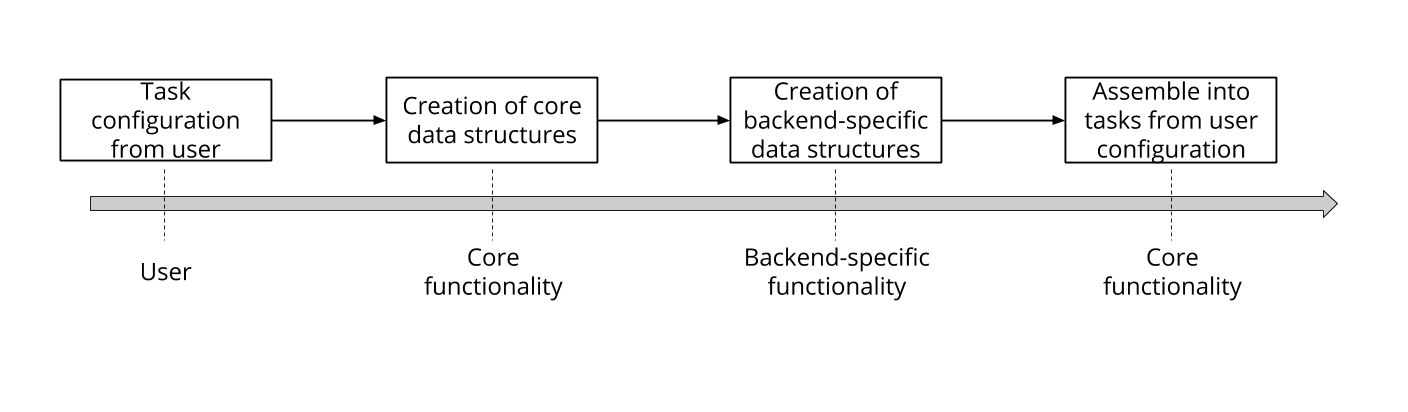
\includegraphics[width=0.9\textwidth]{./chapters/chapter_4/imgs/img_ch4_framework_flow.png}
%%         \caption{Flow of data in the proposed framework}
%%         \label{fig:ch4_proposed_framework_flow}
%%     \end{figure}
%% }

%% \newcommand{\figFrameworkCoreSensor}{
%%     \begin{figure}[!ht]
%%         \centering
%%         \begin{subfigure}[b]{0.3\textwidth}
%%             \centering
%%             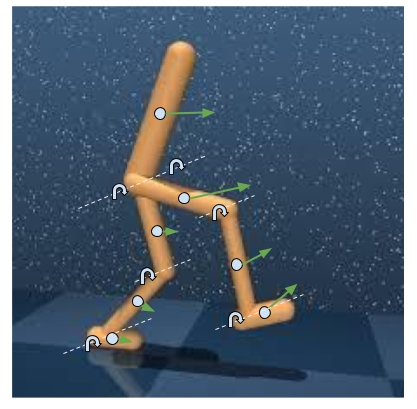
\includegraphics[width=0.9\textwidth]{./chapters/chapter_4/imgs/img_ch4_sensors_core_1.png}
%%             \caption{}
%%             \label{fig:ch4_core_sensor_1}
%%         \end{subfigure}
%%         \begin{subfigure}[b]{0.3\textwidth}
%%             \centering
%%             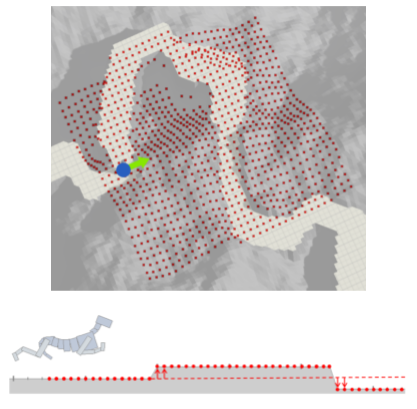
\includegraphics[width=0.9\textwidth]{./chapters/chapter_4/imgs/img_ch4_sensors_core_2.png}
%%             \caption{}
%%             \label{fig:ch4_core_sensor_2}
%%         \end{subfigure}
%%         \begin{subfigure}[b]{0.3\textwidth}
%%             \centering
%%             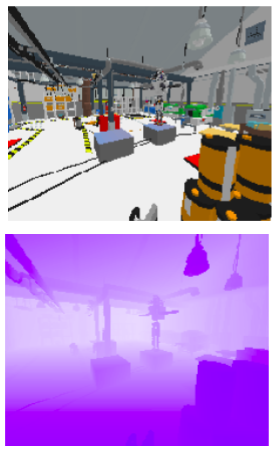
\includegraphics[width=0.9\textwidth]{./chapters/chapter_4/imgs/img_ch4_sensors_core_3.png}
%%             \caption{}
%%             \label{fig:ch4_core_sensor_3}
%%         \end{subfigure}
%%         \caption{Core sensors functionality. a) Intrinsic readings from joints and bodies (adapted from [@CITE]).
%%                                              b) Extrinsic readings from heightmaps of the terrain (adapted from [@CITE,@CITE]).
%%                                              c) Extrinsic readings from rgb and depth images of the agent view (adapted from [@CITE]).}
%%         \label{fig:ch4_core_sensor_functionality}
%%     \end{figure}
%% }

\newcommand{\figPolicyChanges}{
    \begin{figure}[!ht]
        \centering
        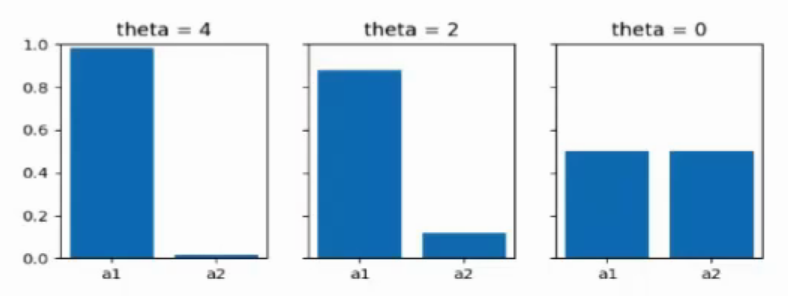
\includegraphics[width=0.8\textwidth]{./chapters/chapter_3/imgs/img_ch3_euclidean_constraint.png}
        \caption{A simple example that shows that same changes in parameter space yield 
                 very different changes in policy space. Adapted from \href{https://youtu.be/yqYKeWtUSO8?t=1050}{this} lecture.}
        \label{fig:ch3_policy_changes}
    \end{figure}
}

\newcommand{\figBenchmarkControlSuite}{
	\begin{figure}
		\centering
		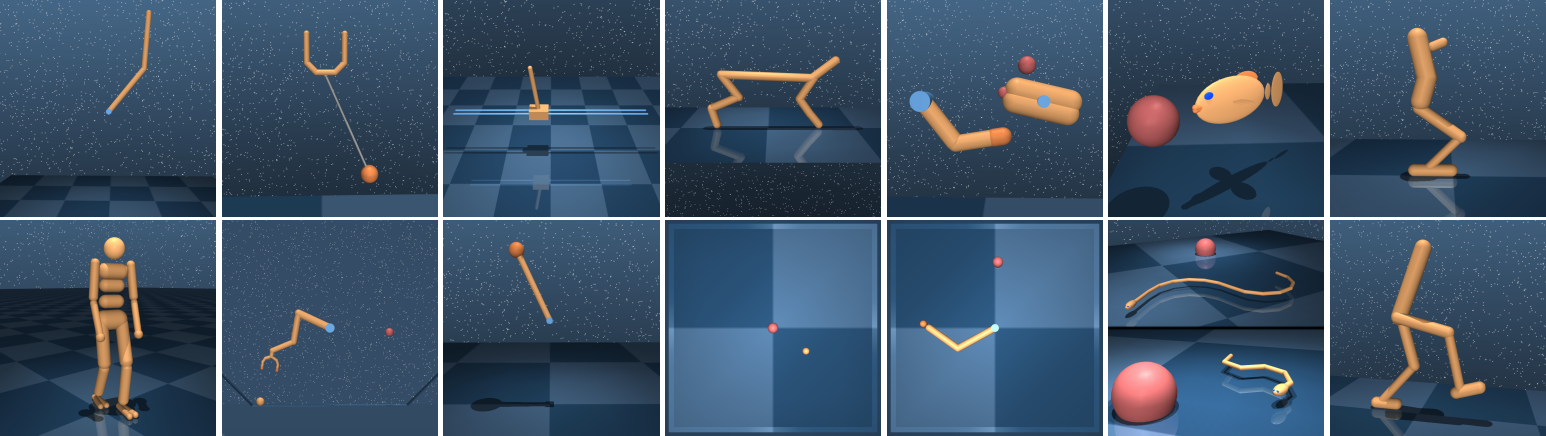
\includegraphics[width=0.9\textwidth]{./chapters/chapter_3/imgs/img_ch3_controlsuite.png}
		\caption{Models available in the Controlsuite benchmark. 
				 Extracted from \citet{Controlsuite}}
	    \label{fig:ch3_controlsuite}
	\end{figure}
}

\newcommand{\figBenchmarkOpenAIGymMujoco}{
    \begin{figure}[!ht]
        \centering
        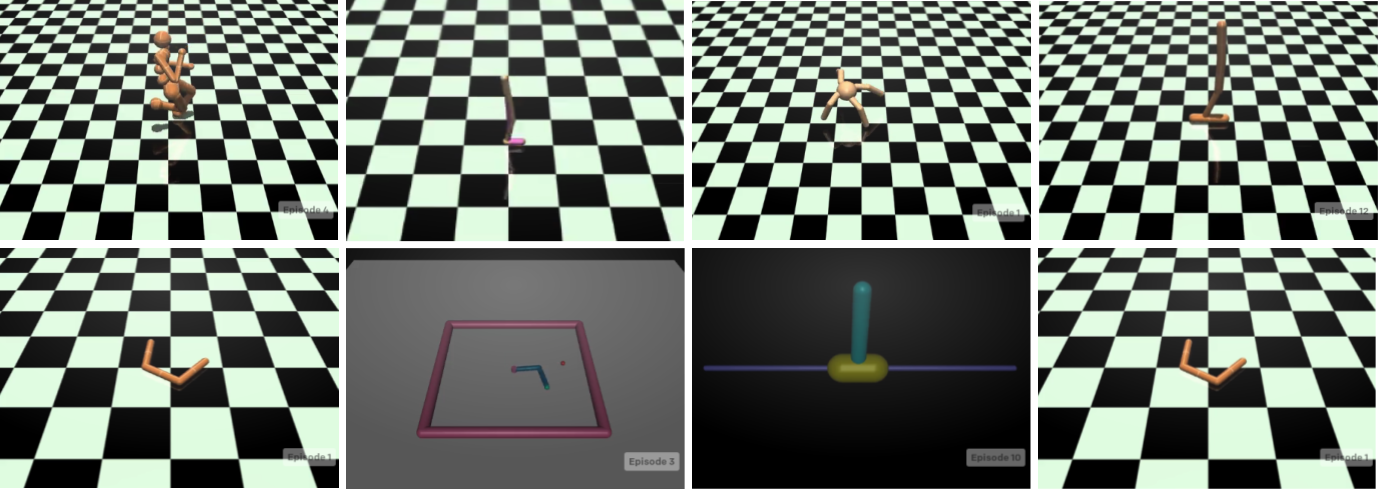
\includegraphics[width=0.9\textwidth]{./chapters/chapter_3/imgs/img_ch3_openaigym_mujoco.png}
        \caption{Models available in the OpenAI-gym benchmark with mujoco as backend. 
                 Extracted from \citet{Gym}}
        \label{fig:ch3_openaigym_mujoco}
    \end{figure}
}

\newcommand{\figBenchmarkOpenAIGymRoboschool}{
    \begin{figure}[!ht]
        \centering
        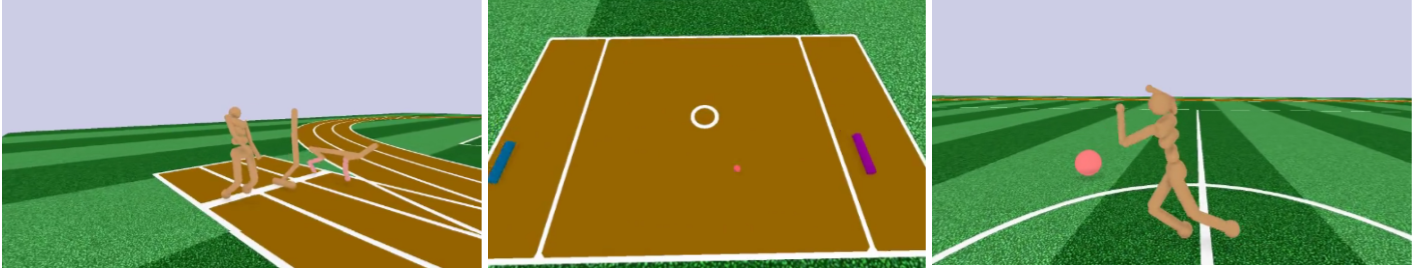
\includegraphics[width=1.0\textwidth]{./chapters/chapter_3/imgs/img_ch3_openaigym_roboschool.png}
        \caption{Models available in the OpenAI-gym benchmark with Bullet as backend. 
                 Extracted from \citet{Roboschool}}
        \label{fig:ch3_openaigym_roboschool}
    \end{figure}
}

\newcommand{\figBenchmarkRllabClassic}{
    \begin{figure}[!ht]
        \centering
        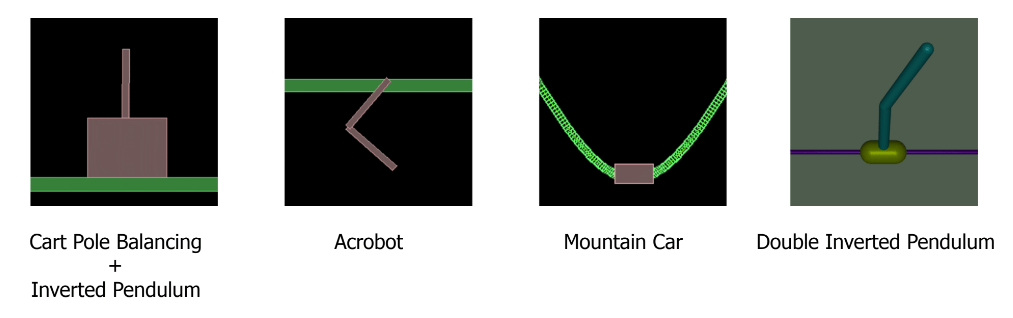
\includegraphics[width=0.9\textwidth]{./chapters/chapter_3/imgs/img_ch3_rllab_classic.png}
        \caption{Models available in the Rllab classic benchmark. Extracted from \cite{Rllab}}
        \label{fig:ch3_rllab_classic}
    \end{figure}
}

\newcommand{\figBenchmarkRllabLocomotion}{
    \begin{figure}[!ht]
        \centering
        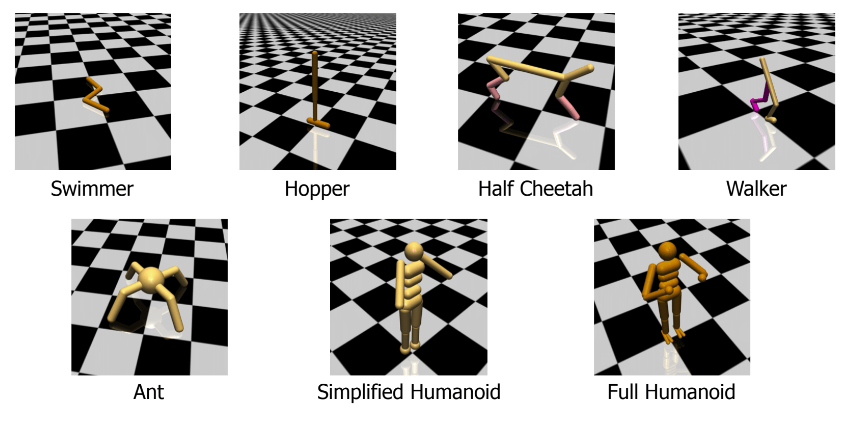
\includegraphics[width=0.9\textwidth]{./chapters/chapter_3/imgs/img_ch3_rllab_locomotion.png}
        \caption{Models available in the Rllab locomotion benchmark. Extracted from \citet{Rllab}}
        \label{fig:ch3_rllab_locomotion}
    \end{figure}
}

\newcommand{\figBenchmarkRllabHierarchical}{
    \begin{figure}[!ht]
        \centering
        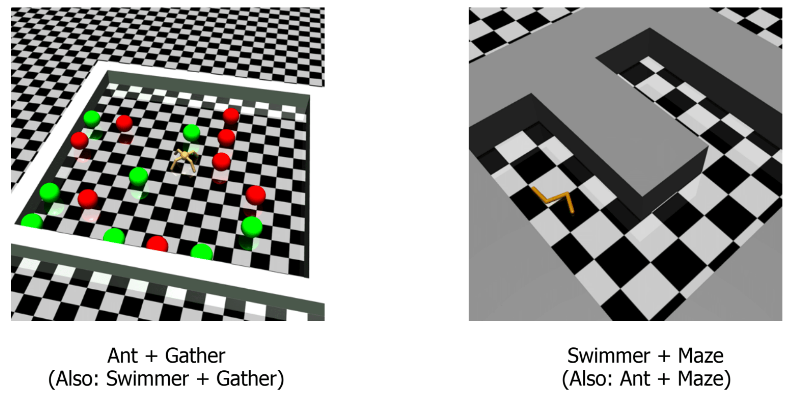
\includegraphics[width=0.9\textwidth]{./chapters/chapter_3/imgs/img_ch3_rllab_hierarchical.png}
        \caption{Models available in the Rllab hierarchical benchmark. Extracted from \citet{Rllab}}
        \label{fig:ch3_rllab_hierarchical}
    \end{figure}
}

\newcommand{\figBenchmarksRobosuite}{
    \begin{figure}[!ht]
        \centering
        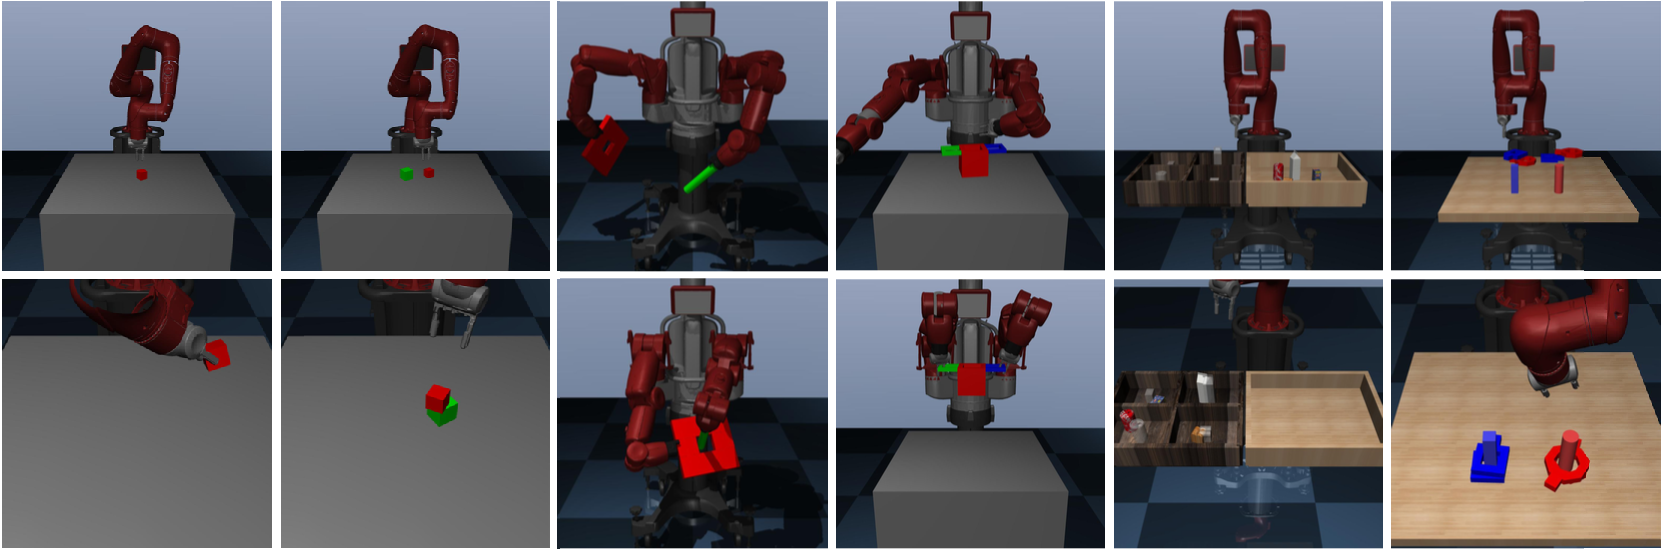
\includegraphics[width=1.0\textwidth]{./chapters/chapter_3/imgs/img_ch3_robosuite.png}
        \caption{Tasks available in Robosuite, as part of the Surreal framework \citep{Surreal}}
        \label{fig:ch3_robosuite}
    \end{figure}
}

\newcommand{\figBenchmarksGpuSim}{
    \begin{figure}[!ht]
        \centering
        \begin{subfigure}[b]{0.3\textwidth}
            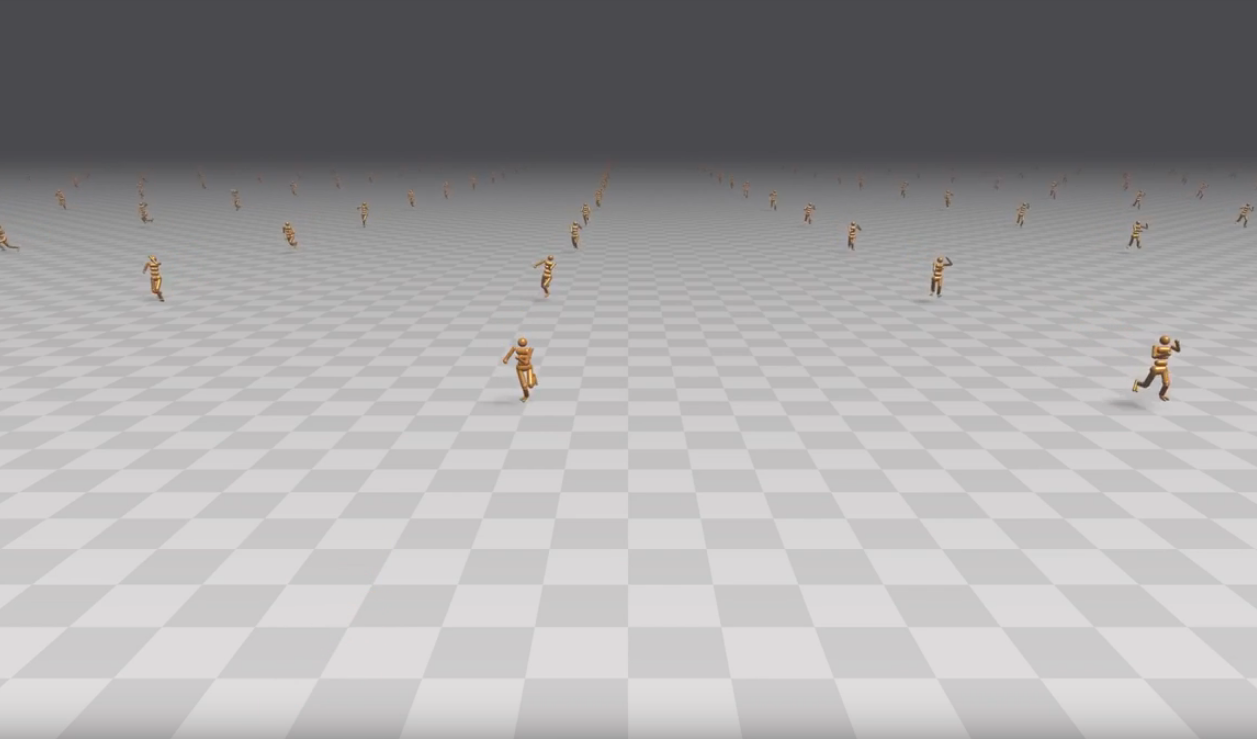
\includegraphics[width=1.0\textwidth]{./chapters/chapter_3/imgs/img_ch3_gpu_sim_1.png}
        \end{subfigure}
        \begin{subfigure}[b]{0.3\textwidth}
            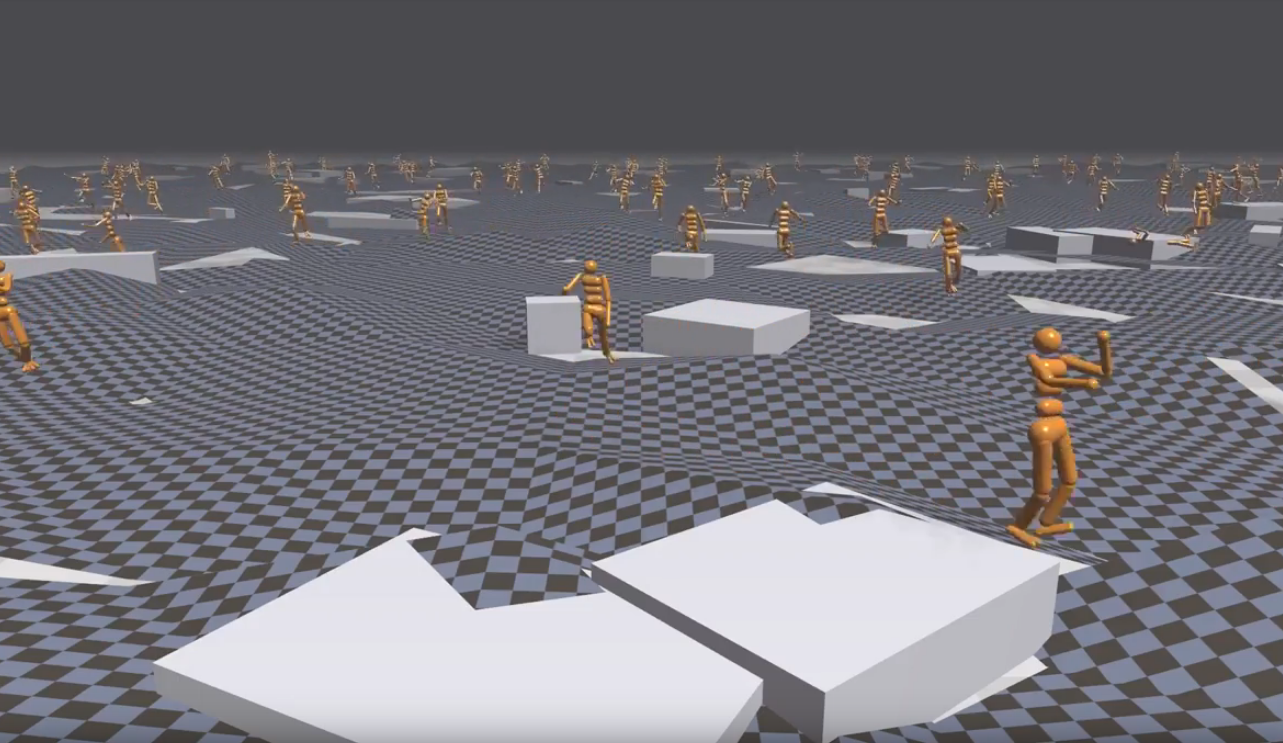
\includegraphics[width=1.0\textwidth]{./chapters/chapter_3/imgs/img_ch3_gpu_sim_2.png}
        \end{subfigure}
        \begin{subfigure}[b]{0.3\textwidth}
            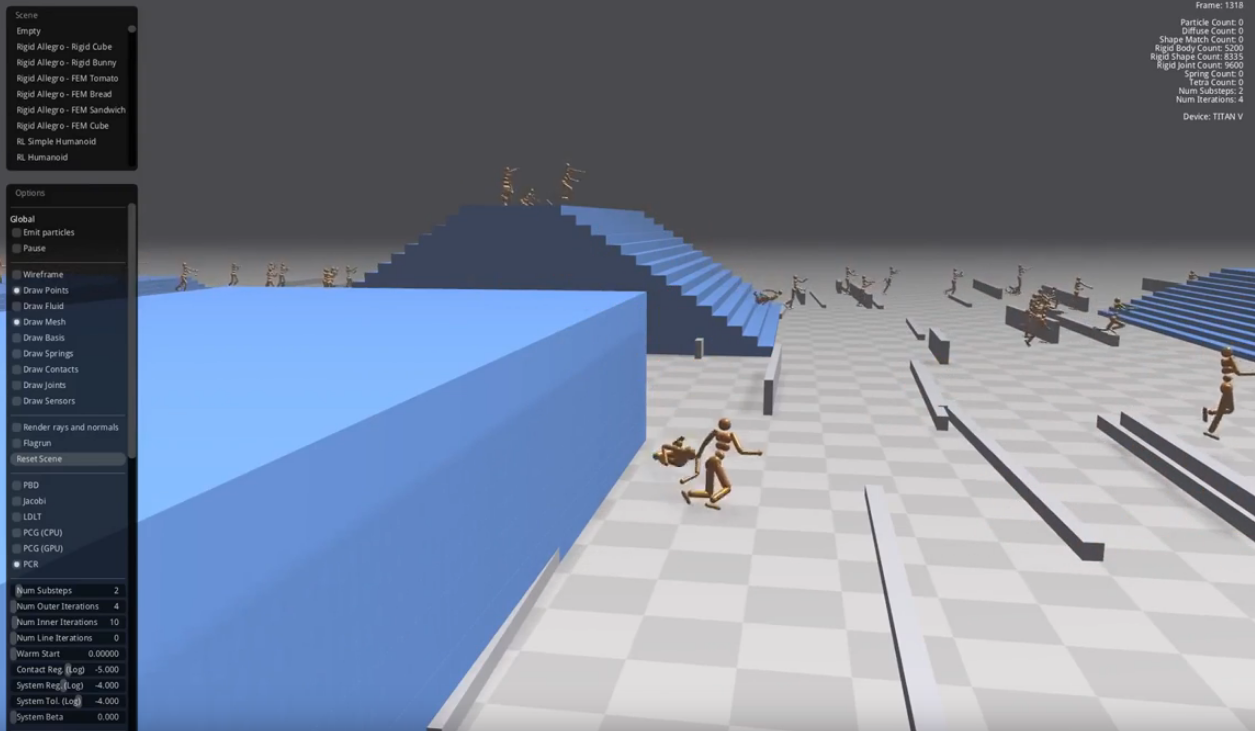
\includegraphics[width=1.0\textwidth]{./chapters/chapter_3/imgs/img_ch3_gpu_sim_3.png}
        \end{subfigure}
        \caption{Tasks provided in the Gpu-Accelerated simulator by \citep{GpuSim}}
        \label{fig:ch3_gpusim}
    \end{figure}
}

\newcommand{\figBenchmarksTerrainRLSim}{
    \begin{figure}[!ht]
        \centering
        \begin{subfigure}[b]{0.3\textwidth}
            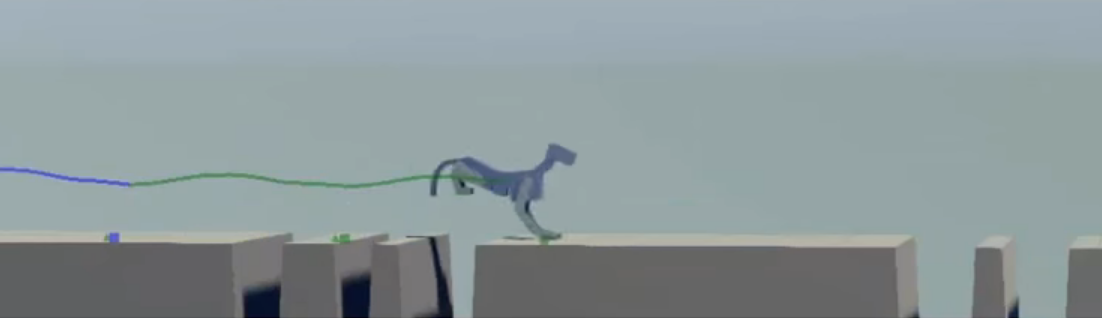
\includegraphics[width=1.0\textwidth]{./chapters/chapter_3/imgs/img_ch3_terrainrlsim_1.png}
            \caption{}
        \end{subfigure}
        \begin{subfigure}[b]{0.3\textwidth}
            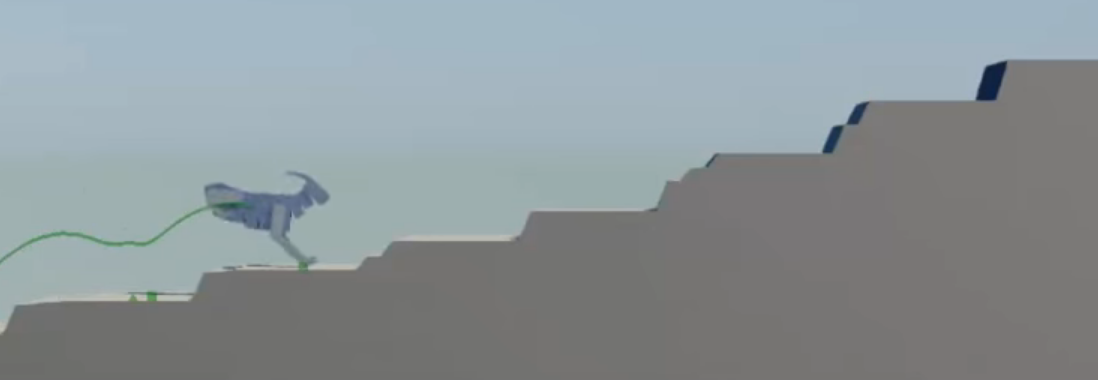
\includegraphics[width=1.0\textwidth]{./chapters/chapter_3/imgs/img_ch3_terrainrlsim_2.png}
            \caption{}
        \end{subfigure}
        \begin{subfigure}[b]{0.3\textwidth}
            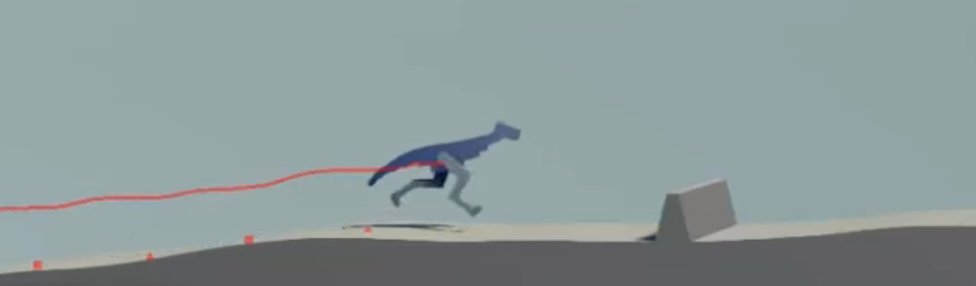
\includegraphics[width=1.0\textwidth]{./chapters/chapter_3/imgs/img_ch3_terrainrlsim_3.png}
            \caption{}
        \end{subfigure}

        \centering
        \begin{subfigure}[b]{0.3\textwidth}
            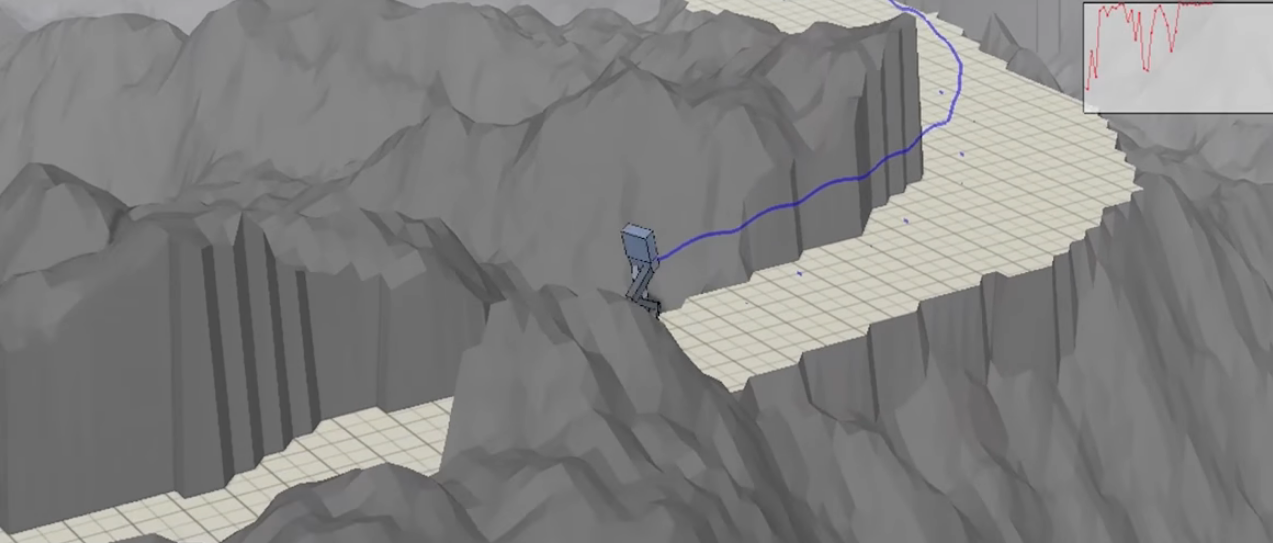
\includegraphics[width=1.0\textwidth]{./chapters/chapter_3/imgs/img_ch3_terrainrlsim_4.png}
            \caption{}
        \end{subfigure}
        \begin{subfigure}[b]{0.3\textwidth}
            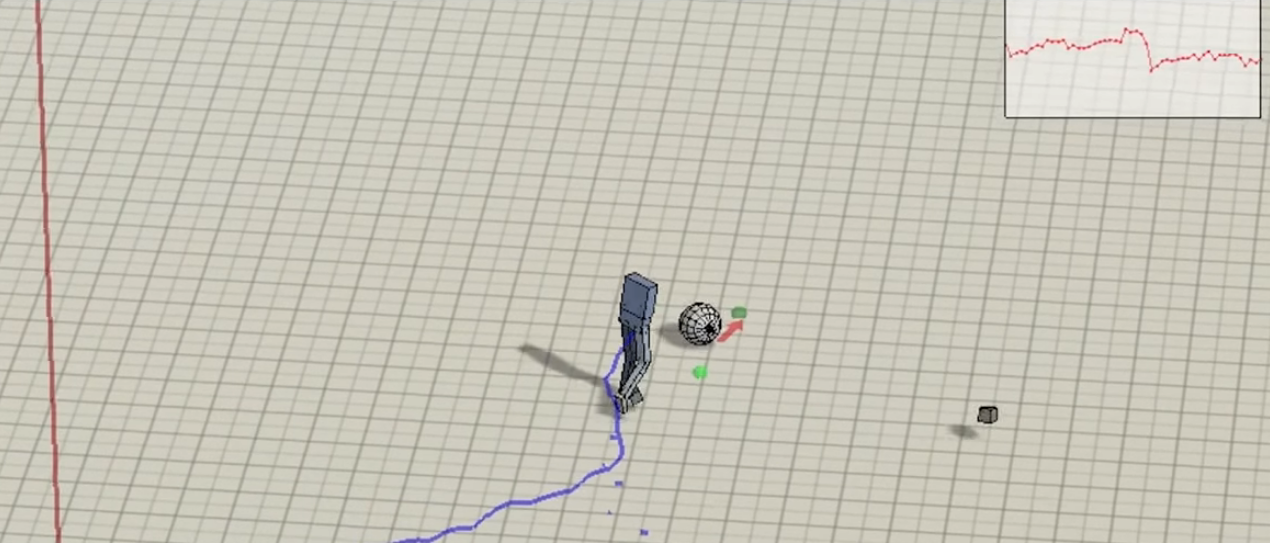
\includegraphics[width=1.0\textwidth]{./chapters/chapter_3/imgs/img_ch3_terrainrlsim_5.png}
            \caption{}
        \end{subfigure}
        \begin{subfigure}[b]{0.3\textwidth}
            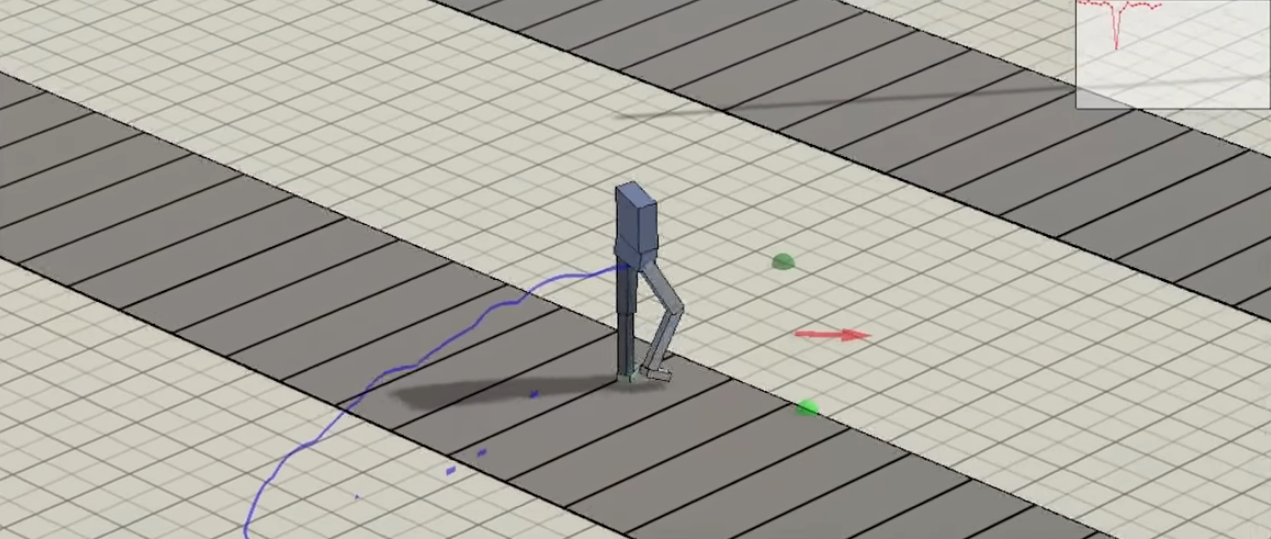
\includegraphics[width=1.0\textwidth]{./chapters/chapter_3/imgs/img_ch3_terrainrlsim_6.png}
            \caption{}
        \end{subfigure}

        \centering
        \begin{subfigure}[b]{0.3\textwidth}
            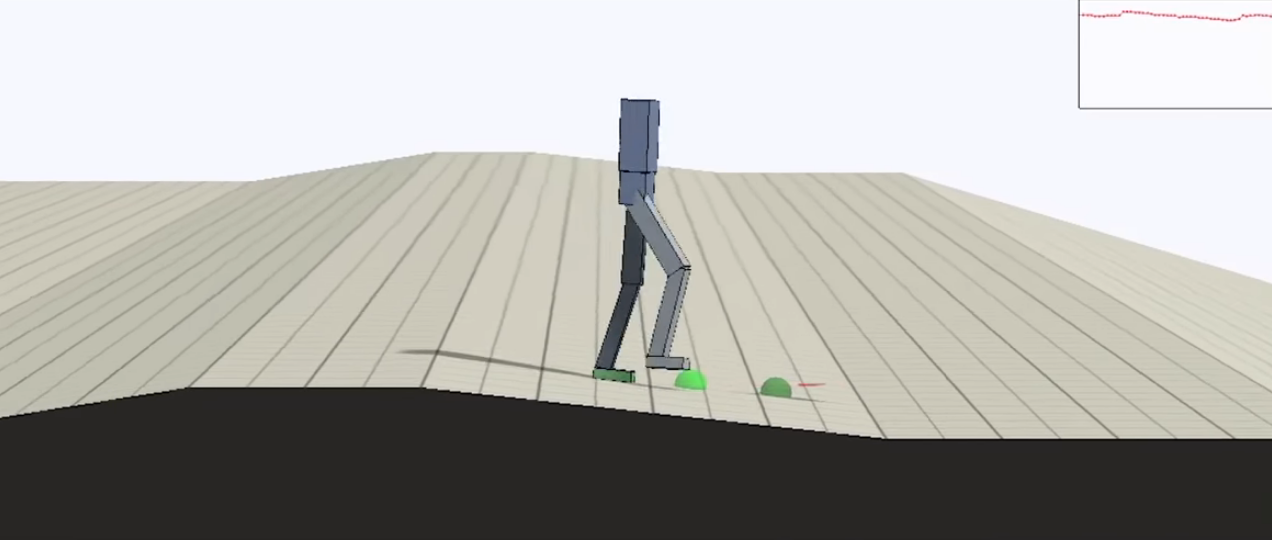
\includegraphics[width=1.0\textwidth]{./chapters/chapter_3/imgs/img_ch3_terrainrlsim_7.png}
            \caption{}
        \end{subfigure}
        \begin{subfigure}[b]{0.3\textwidth}
            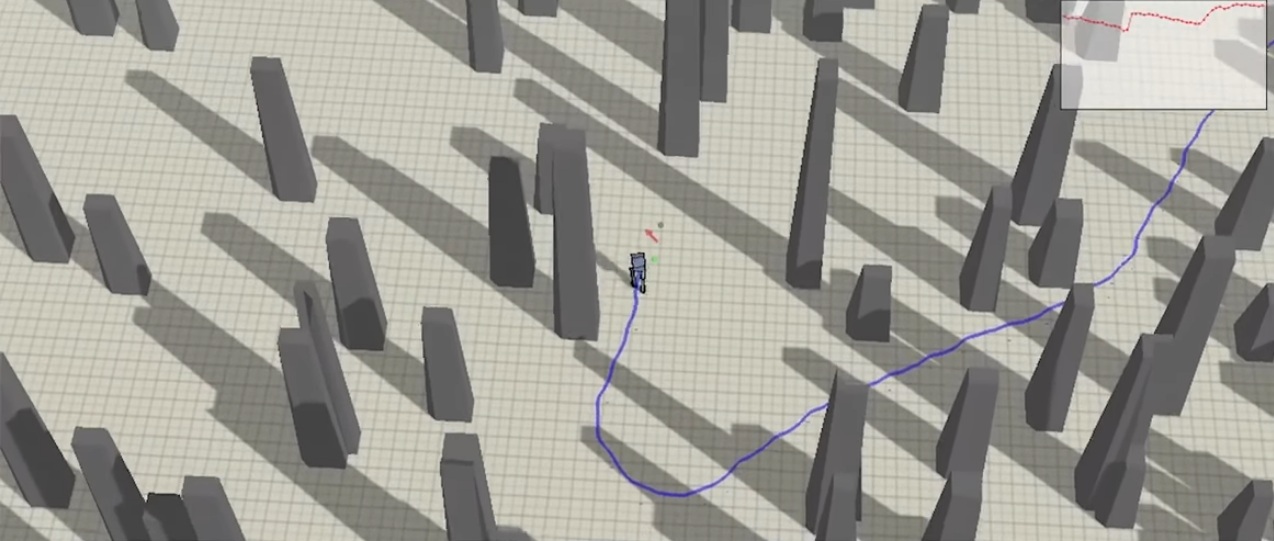
\includegraphics[width=1.0\textwidth]{./chapters/chapter_3/imgs/img_ch3_terrainrlsim_8.png}
            \caption{}
        \end{subfigure}
        \begin{subfigure}[b]{0.3\textwidth}
            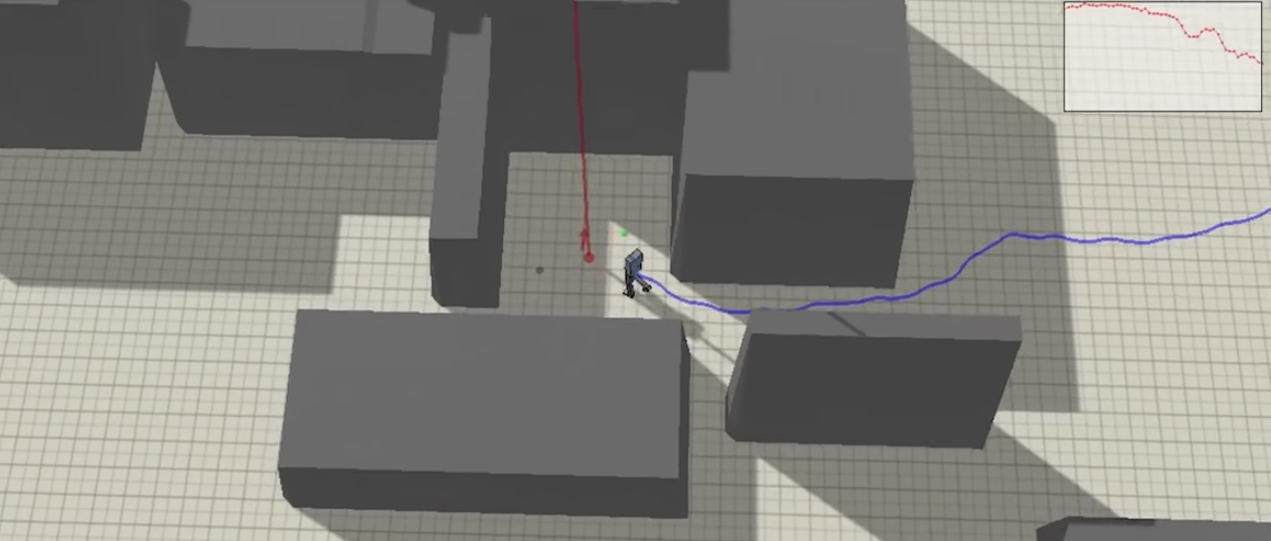
\includegraphics[width=1.0\textwidth]{./chapters/chapter_3/imgs/img_ch3_terrainrlsim_9.png}
            \caption{}
        \end{subfigure}

        \centering
        \begin{subfigure}[b]{0.3\textwidth}
            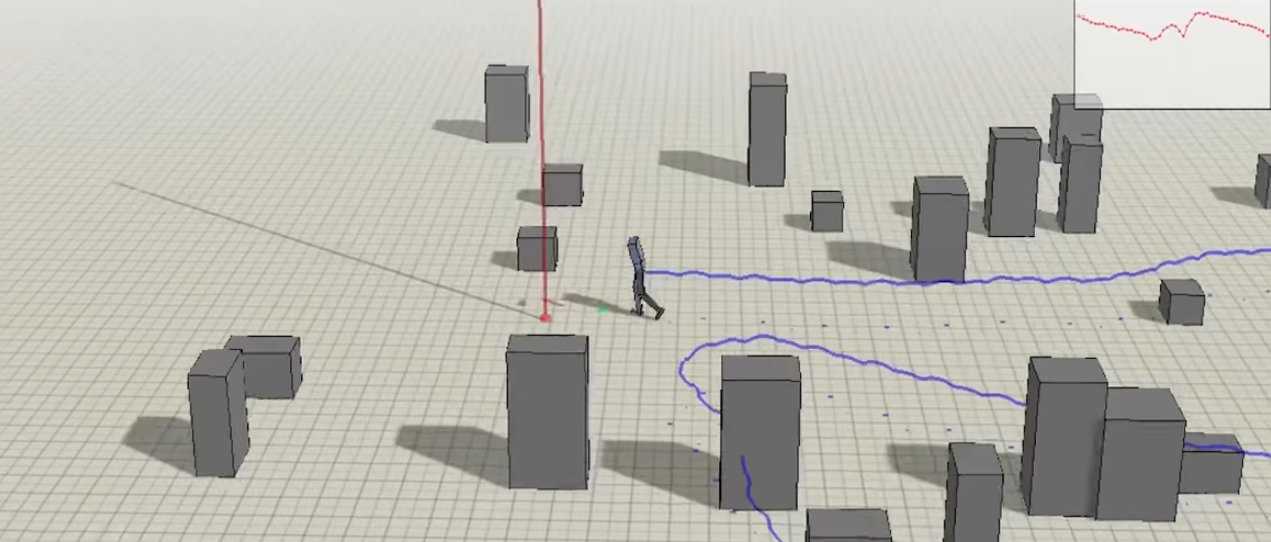
\includegraphics[width=1.0\textwidth]{./chapters/chapter_3/imgs/img_ch3_terrainrlsim_10.png}
            \caption{}
        \end{subfigure}

        \caption{Some of the tasks provided by the TerrainRLSim benchmark.}
        \label{fig:ch3_terrainrlsim}
    \end{figure}
}

\newcommand{\figBenchmarksUnityMLAgents}{
    \begin{figure}[!ht]
        \centering
        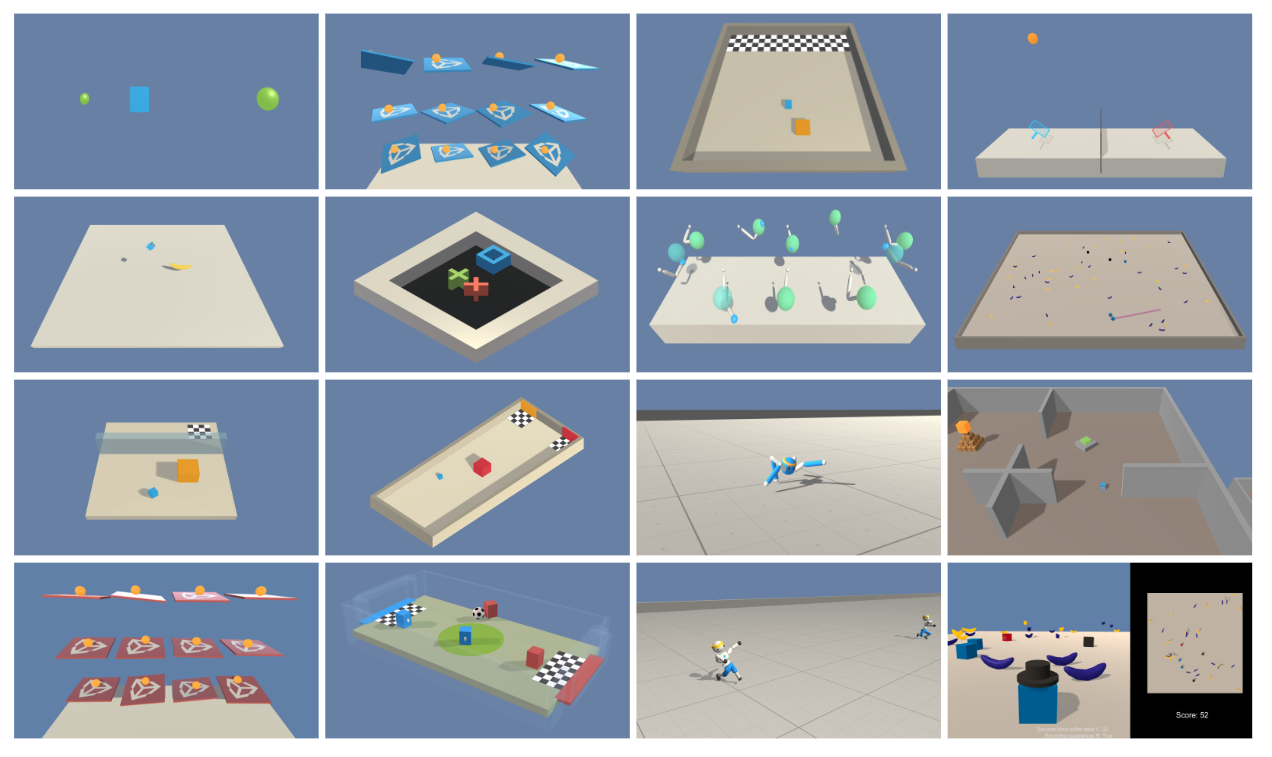
\includegraphics[width=1.0\textwidth]{./chapters/chapter_3/imgs/img_ch3_unity_ml_agents.png}
        \caption{Tasks available in the Unity ML-Agents framework.}
        \label{fig:ch3_unity_ml_agents}
    \end{figure}
}

\newcommand{\figBenchmarksMarathonEnvs}{
    \begin{figure}[!ht]
        \centering
        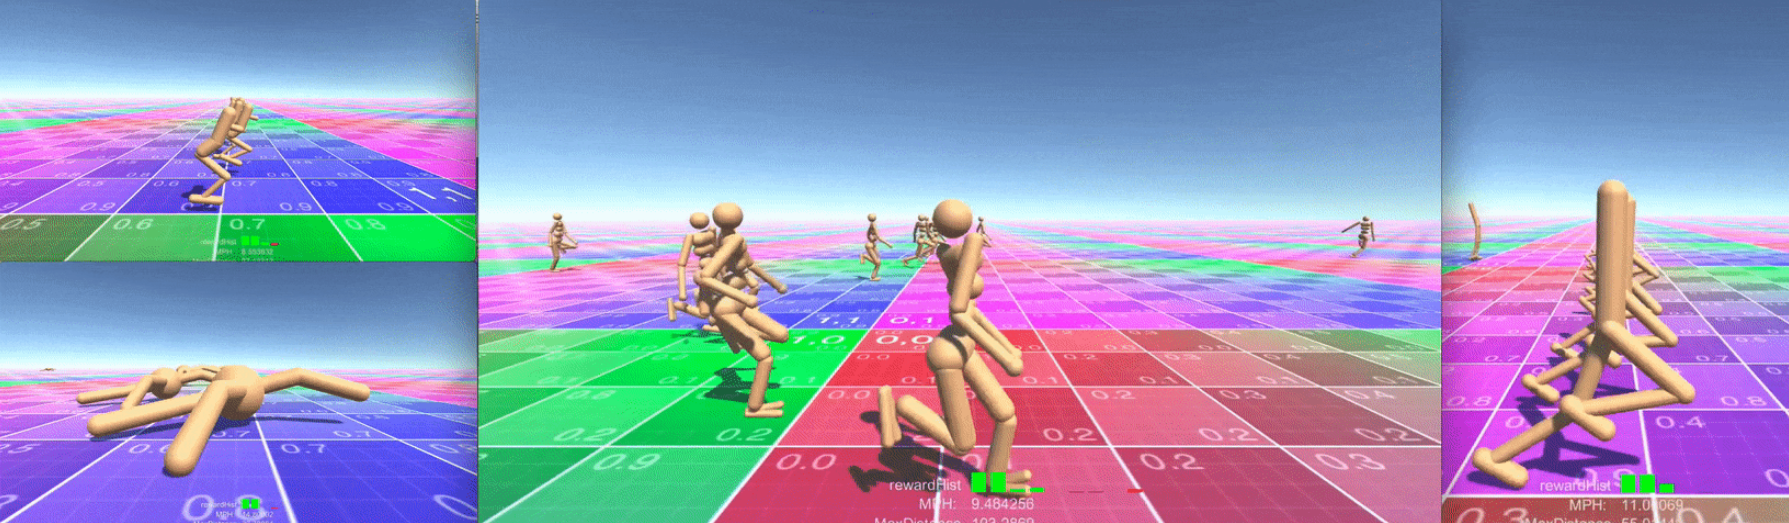
\includegraphics[width=1.0\textwidth]{./chapters/chapter_3/imgs/img_ch3_marathon_envs.png}
        \caption{Tasks available in the Marathon benchmark, provided along with the Unity ML-Agents framework.}
        \label{fig:ch3_marathon_envs}
    \end{figure}
}
%%%%%%%%%%%%%%%%%%%%%%%%%%%%%%%
%   Algorithms for chapter 3
%%%%%%%%%%%%%%%%%%%%%%%%%%%%%%%

\todo{Me preocupa un poco que la revision sea solo de herramientas, osea está muy orientado a eso, puede ser un punto en contra para un evaluador}

In this chapter we will give an overview of current state of the art DeepRL algorithms
used in locomotion tasks, which will be the baselines we will evaluate with the proposed
framework. We also discuss various recent works in locomotion which also apply 
these algorithms. Finally we give an overview of the current benchmarks being
used for locomotion tasks.

\section{Deep RL algorithms for locomotion} \label{sec:ch3_deeprl_algorithms}

Current state of the art DeepRL algorithms used in locomotion tasks are \textbf{Policy Based} 
algorithms (or variants), which were introduced in section ~\ref{ref:subs:ch2:PolicyBasedMethods}. 
These variants address various problems with the standard Vanilla Policy Gradient algorithm,
which include:

\begin{itemize}
    \item \textbf{Step size selection}: The step size is of major importance in DeepRL,
          because the data the agent gets, which is then used for learning, is obtained
          using the policy, which is changed every gradient update step. Besides, the advantage
          signal that we estimate is very noisy, and this can lead to bad updates.

    \item \textbf{Sample efficiency}: The vanilla version of policy gradients uses
          the sampled data for only a single gradient estimation and update. This is
          very inefficient because the data sampled from the environment usually involves
          running the simulation for various episodes, which in some cases is very 
          computationally expensive.
\end{itemize}

To address these issues one approach is to turn the RL problem into a small 
optimization problem for each policy update. One simple way to achieve this
result is to use the loss function from ~\ref{eq:ch2_vpg_loss}, which allows to
reuse the collected data as much as possible until convergence. This results
in the following small optimization problem.

\begin{equation}
    \theta_{new} = \arg \max_{\theta} \mathbb{\hat E}_{t} 
                        \left [
                            \log \pi_{\theta}(a_{t}|s_{t}) \hat A_{t}
                        \right ]
\end{equation}

Unfortunately we cannot use this update until convergence, because of the issues
mentioned before. To avoid updating the policy too much we place a constraint in
the optimization problem by forcing small changes in the policy parameters. We also
makes a change in the loss function, and instead of using the simpler loss $L^{PG}$
we use a loss $L^{IS}$, which is derived using importance sampling (both result in
the same gradient). This results in the following constrained optimization problem.

\begin{align}
    \theta_{new} = \arg \max_{\theta} \mathbb{\hat E}_{t} 
                        \left [
                            \frac{\pi_{\theta}(a_{t}|s_{t})}
                                 {\pi_{\theta_{old}}(a_{t}|s_{t})} \hat A_{t}
                        \right ] \nonumber \\
    \textit{subject to: } 
                \Vert \theta - \theta_{old} \Vert_{2} \leq \delta
\end{align}

Even though we have a constrained the optimization problem with an threshold in the
eucliden distance of the policy parameters, this usually does not yield the desired
results. For example, suppose we have a stochastic policy over a discrete action
space of two actions, parameterized using a single parameter  $\theta$ and a sigmoid 
function $\sigma$ in the following form.

\begin{gather*}
    \pi_{\theta}(a) = 
            \begin{cases}
                \sigma(\theta)          & a = 1 \\
                1 - \sigma({\theta})    & a = 2
            \end{cases}
\end{gather*}

Two fixed changes in the policy parameter $\theta$ give very different changes in
the output probabilities of the policy. The following figure shows this issue for
the case of $\Delta \theta=2$, applied in $\theta$ 0, 2 and 4.

\figPolicyChanges

\subsection{Natural Policy Gradients}

A better policy update was proposed by \cite{NaturalPolicyGradient}, in which
the authors proposed using the natural gradient instead of the a simple gradient 
update.

\begin{equation}
    \tilde{\nabla}_{\theta} J(\theta) = F^{-1}(\theta) \nabla_{\theta} J(\theta)
\end{equation}

This update makes use of the \textit{Fisher Information Matrix} $F$, which is used
to compensate the effects mentioned previously. This update also arises by reformulating
the small optimization problem into the following form:

\begin{align} \label{eq:}
    \theta_{new} = \arg \max_{\theta} \mathbb{\hat E}_{t} 
                        \left [
                            \frac{\pi_{\theta}(a_{t}|s_{t})}
                                 {\pi_{\theta_{old}}(a_{t}|s_{t})} \hat A_{t}
                        \right ] \nonumber \\
    \textit{subject to: } 
                \bar{D}_{KL}(\theta||\theta_{old}) \leq \delta
\end{align}

The only difference is the change of the euclidean constraint in parameter space
to the constraint in the KL-divergence of the parameterized probability distributions,
which ensures that the changes in parameter space made do not change the resulting 
distribution over action drastically. By solving this optimization problem using
linearization (Taylor Expansions) we obtain the following algorithm.

\algNaturalPolicyGradients

\subsection{Trust Region Policy Optimization (TRPO)}

The previous algorithm requires the inversion of the Fisher information matrix, which
is costly depending on the size of the parameters space (how big is the function approximator).
Also, it does not give theoretical improvement guarantees about the results, although
it provided better updates than the Vanilla Policy Gradient. \cite{TRPO} introduced
important changes that allow to solve the inversion issue, and also provided theoretical 
improvement guarantees on the policy updates (each update is guaranteed to improve performance).
The changes they introduced are listed below, and the resulting algorithm in shown in
Algorithm ~\ref{alg:trpo}.

\begin{itemize}
    \item Use the \textbf{conjugate gradient method} to avoid computing the inverse.
    \item Perform \textbf{line search} in the step size to make the largest update
          that satisfies the KL constraint.
\end{itemize}

\algTRPO

Some results (from the authors) of this algorithm in locomotion tasks and video game playing tasks 
can be found in the following \href{https://youtu.be/jeid0wIrSn4}{link}.

\subsection{Proximal Policy Optimization (PPO)}

This algorithm was introduced by \cite{PPO}, and it also tries to make the biggest
update possible while satisfying the same constraints and using all the data collected
for that optimization step. The authors proposed a simpler algorithm that requires
only an optimization over a surrogate loss function that approximates the behaviour
of the KL constraint. This loss in shown in the following equation. 

\begin{equation}
    L^{CLIP}(\theta) = \min \left ( \frac{\pi_{\theta}(a|s)}{\pi_{\theta_{old}}(a|s)} A^{\pi_{old}},
                                clip \left ( 
                                \frac{\pi_{\theta}(a|s)}{\pi_{\theta_{old}}(a|s)},
                                1-\epsilon, 1+\epsilon
                                     \right ) A^{\pi_{old}} \right )
\end{equation}

By using this loss in the optimization problem the resulting algorithm solves a similar
objective to TRPO, but without formulating the constrained optimization problem nor
using second order optimization, which is slightly costly in the TRPO implementations.
The resulting algorithm is shown below.

\algPPO

Some results (from the authors) of this algorithm in locomotion tasks and video game playing tasks 
can be found in the following \href{https://blog.openai.com/openai-baselines-ppo/}{link}.

\newpage

\section{DeepRL applied to locomotion}

In this last section we discuss current state of the art results of DeepRL in
locomotion tasks. These served as the inspiration for this proposal to the extent
that most of this proposal serves as an extension of these results to more 
diverse and complicated environments.


\subsection{Benchmarking DeepRL for Continuous Control}


\subsection{DeepTerrainRL}


\subsection{DeepLoco}


\subsection{Emergence of Locomotion}


\subsection{DeepMimic}

\newpage

\section{DeepRL locomotion benchmarks}

\subsection{Deepmind ControlSuite}

This set of benchmarks was first introduced in \cite{Controlsuite}, and consists 
of various locomotion tasks (shown in Figure ~\ref{fig:ch3_controlsuite}), with various types of agents 
to select from. The models available consist of xml files in the mujoco format (mjcf) 
that are used as the blueprints to instantiate an agent. The tasks consist of the specific
setups that the agents must solve, like walking, standing, running, etc.

\figBenchmarkControlSuite

As described in their \href{https://arxiv.org/pdf/1801.00690.pdf}{technical report},
some of the key features of this benchmark include:

\begin{itemize}
    \item \textbf{Full state observations}: the observations provided to the agent
          are sufficient to recover the full state of the environment. These observations
          include positions and velocities (of bodies and joints), touch sensor readings,
          and some other task specific measurements. Using this information, the full state
          of the environment can be recovered due to the simple nature of the environment 
          (most locomotion tasks in the benchmark are flat terrain tasks, and no information
          is hidden from the agents).

    \item \textbf{Normalized actions}: the actions exposed to the user have been normalized 
          in the range $\left[-1,1\right]$. These are mapped to actuators that represent
          torques applied to joints (torque actuation model).

    \item \textbf{Normalized rewards}: the rewards are set to the range $\left[ 0, 1 \right]$, 
          and can be smooth (whole range) or sparse (just the values $\left\{0,1\right\}$).

    \item \textbf{MuJoCo backend}: MuJoCo is the underlying physics backend, and it is
          integrated into the suite by using Python bindings generated using 
          \href{https://github.com/deepmind/dm_control/blob/master/dm_control/autowrap/autowrap.py}{ctypes}.
\end{itemize}

\subsection{OpenAI Gym}

This set of benchmarks consists of two separate options depending on the physics 
backend (MuJoCo and Bullet). These two options are Python Wrappers for the supported 
physics backends and are used as low level functionality for the high level API provided by Gym \citep{Gym}.
The options used as wrappers for the two physics backends available are the following:

\begin{itemize}
    \item \textbf{Mujoco-py} : A Python wrapper for MuJoCo, very similar to ControlSuite. 
          The available tasks are similar to the ones in ControlSuite, which are shown 
          in Figure ~\ref{fig:ch3_openaigym_mujoco}.

        \figBenchmarkOpenAIGymMujoco

    \item \textbf{RoboSchool}: An implementation that uses PyBullet, which exposes 
          the Bullet physics engine through a Python API. The environments exposed 
          are a bit different to the previous suite, and are shown in Figure ~\ref{fig:ch3_openaigym_roboschool}. 

        \figBenchmarkOpenAIGymRoboschool

\end{itemize}

The RL API exposed by Gym is similar to the one exposed by ControlSuite. 
In each step taken in the environment, the API returns the observation, 
reward, and some extra observations. More information can be found in its 
technical report \citep{Gym}, and in its \href{https://github.com/openai/gym}{repository}.

\subsection{Rllab and Garage}

Rllab is a set of benchmarks similar to the previous two. It implements its own 
Python wrapper for MuJoCo, and builds its own Reinforcement Learning API on top 
of that wrapper. It provides a set of tested baselines of various Deep Reinforcement 
Learning algorithms, which were presented in \cite{Rllab}. The environments provided 
by Rllab are grouped in three categories: \textbf{classic} (Figure ~\ref{fig:ch3_rllab_classic}), 
\textbf{locomotion} (Figure ~\ref{fig:ch3_rllab_locomotion}) and \textbf{hierarchical} 
(Figure ~\ref{fig:ch3_rllab_hierarchical}). It is compatible with Gym, by means of 
a wrapper on top of its environments, but as they explain in their documentation 
\href{https://rllab.readthedocs.io/en/latest/user/gym_integration.html}{website} 
this is a very different API.

\figBenchmarkRllabClassic

\figBenchmarkRllabLocomotion

\figBenchmarkRllabHierarchical

Garage is the next version of the Rllab suite, and is very similar in architecture 
to Rllab, with support for more environments and baselines. To this date the number 
of environments is similar to the ones in Rllab, but is being actively supported, 
compared to Rllab. More information can be found in its \href{https://github.com/rlworkgroup/garage}{repo}.

\subsection{Robosuite}
 
\href{https://github.com/StanfordVL/robosuite/}{Robosuite} is a set of benchmarks first 
introduced along the \href{https://surreal.stanford.edu/}{Surreal} 
framework by \cite{Surreal}. This set of benchmarks is more oriented towards robot manipulation,
providing tasks that involve robot models commonly used as robotics manipulation research platforms 
(like \textit{sawyer} and \textit{baxter}).

This set of benchmarks use MuJoCo as physics backend (through mujoco-py), and as they
explain in their documentation, the suite provides various APIs that allow the user
to create diverse experiments. By using its programmatical task construction API
the user can create an specific setup with just a few lines of Python code.
The tasks provided in the suite are shown in Figure ~\ref{fig:ch3_robosuite}.

\figBenchmarksRobosuite

\subsection{Gpu-Accelerated Simulation}

This set of benchmarks was presented in \cite{GpuSim}, and makes use of a custom 
physics backend developed in-house. The physics simulator is built on top of the 
NVIDIA FleX physics engine, which focuses on accelerated GPU physics simulation. 
This approach allows to run scenes with a large number of agents, ranging in the 
thousands. One key detail to consider is the usage of FleX, which is a position 
based dynamics engine. This type of simulations allows for fast simulation by trading
accuracy. 

The simulator is not yet released (as stated by the authors, it is still 
work in progress), but will probably be released as part of the 
\href{https://developer.nvidia.com/isaac-sdk}{NVIDIA Isaac platform}. Some of the 
benchmarks presented are shown in Figure ~\ref{fig:ch3_gpusim}, and include tasks
involving hundreds of humanoids running in environments from low to high complexity.

\figBenchmarksGpuSim

\subsection{TerrainRLSim}

This set of benchmarks was presented in \cite{TerrainRLSim}, and was used in \cite{DeepTerrainRL}, 
\cite{ActuationChoice} as the core framework. This suite uses Bullet as physics backend,
and one key difference with the other presented works is the diversity of the tasks provided.
The tasks provided are shown in Figure ~\ref{fig:ch3_terrainrlsim}, and range from 
single direction obstacle courses, to two dimensional traversal tasks.

\figBenchmarksTerrainRLSim

\subsection{Unity ML-Agents}

This set of benchmarks was presented in \cite{UnityMLAgents}, and it is a framework 
built on top the \citeauthor{Unity} game engine, which makes use of PhysX as backend. 
The tasks are ports of various tasks from the previous benchmarks, and can be used
through a Python API that connects to the games that represent the tasks. The base tasks
provided by the framework are shown in Figure ~\ref{fig:ch3_unity_ml_agents}. Also, 
there are a set of tasks that are provided on top of this framework through the 
\href{https://github.com/Unity-Technologies/marathon-envs}{Marathon Environments} 
package, and are shown in Figure ~\ref{fig:ch3_marathon_envs}.

\figBenchmarksUnityMLAgents

\figBenchmarksMarathonEnvs